\documentclass{article}

\usepackage[utf8]{inputenc}
\usepackage{enumerate}
\usepackage{graphicx}
\usepackage[spanish]{babel}
\usepackage{bm}

\title{\textbf{Mecánica computacional - Trabajo Práctico 2}}
\author{FILARDI, Esteban; VICTORIO, Franco}
\date{}

\def\intone{\int_{-1}^1}
\def\dx{\mbox{d}x}
\def\dy{\mbox{d}y}
\def\domega{\mbox{d}\Omega}
\def\dgamma{\mbox{d}\Gamma}
\def\summ{\sum_{m=1}^M}
\def\partialx#1{\frac{\partial #1}{\partial x}}
\def\partialy#1{\frac{\partial #1}{\partial y}}
\def\partialxx#1{\frac{\partial^2 #1}{\partial x^2}}
\def\partialyy#1{\frac{\partial^2 #1}{\partial y^2}}
\def\hatsigmax{\hat{\sigma}_x}
\def\hatsigmay{\hat{\sigma}_y}
\def\hattauxy{\hat{\tau}_{xy}}

\begin{document}

\maketitle

\begin{enumerate}[1)]
    \item{ % 1)
        En los dos casos se usa:

        \[ \psi = x + 1 \]
        \[ N_m(x) = \sin(m \pi x) \]

        El error utilizado es:

        \[ \mbox{error} = \frac{\left|\left| x_{aprox} - x_{exacta}\right|\right|_2}{\left|\left| x_{exacta} \right|\right|_2} \]

        evaluando en $1000$ puntos equiespaciados en $[0, 1]$.

        \vspace{0.5cm}

        \textbf{Colocación puntual}: usando $M$ puntos equiespaciados
        y en el interior del dominio (para $M=2$ los puntos 
        $\frac{1}{3}$ y $\frac{2}{3}$, por ejemplo), se obtienen los
        siguientes resultados:

        \begin{tabular}{|c|c|c|}
        \hline
        \textbf{M} & \textbf{Error} & \textbf{Proporción mejora} \\
        \hline
        1 & 5.1067e-01 & \\
        \hline
        2 & 1.6125e-01 & 3.1670 \\
        \hline
        4 & 4.1164e-02 & 3.9173 \\
        \hline
        8 & 9.1047e-03 & 4.5212 \\
        \hline
        16 & 1.8320e-03 & 4.9697 \\
        \hline
        32 & 3.4760e-04 & 5.2706 \\
        \hline
        \end{tabular}

        \vspace{0.5cm}

        \textbf{Galerkin}: con el método de Galerkin se obtienen
        los siguientes resultados:

        \begin{tabular}{|c|c|c|}
        \hline
        \textbf{M} & \textbf{Error} & \textbf{Proporción mejora} \\
        \hline
        1 & 9.4531e-03 & \\
        \hline
        2 & 2.8715e-03 & 3.2921 \\
        \hline
        4 & 6.8859e-04 & 4.1701 \\
        \hline
        8 & 1.4254e-04 & 4.8309 \\
        \hline
        16 & 2.7272e-05 & 5.2267 \\
        \hline
        32 & 5.0146e-06 & 5.4384 \\
        \hline
        \end{tabular}

        \vspace{0.5cm}

        A continuación se muestran las gráficas para ambos métodos en el
        caso $M=2$:

        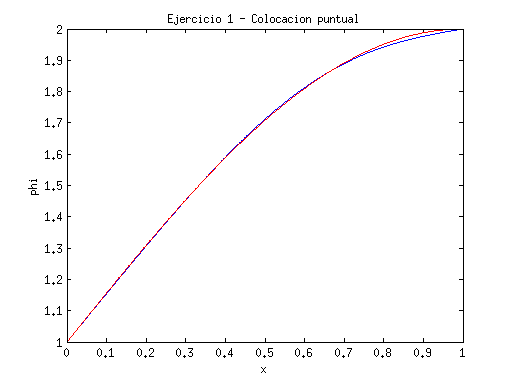
\includegraphics[width=\textwidth]{ej1_cp.png}

        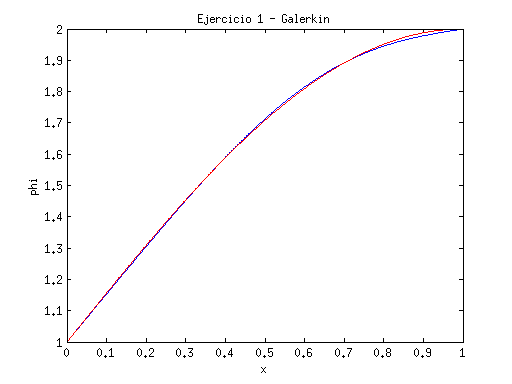
\includegraphics[width=\textwidth]{ej1_galerkin.png}
    }
    \item{ % 2)
        La solución exacta al problema dado es:

        \[ \phi(x) = \frac{1 + \sin(1) - \cos(1)}{\cos(1) + \sin(1)} \sin(x) + \cos(x) - 1 \]

        Usando el método de los resiudos ponderados puede obtenerse una solución aproximada
        de la forma $\psi + \sum_{m=1}^M a_m N_m$. Dado que hay una condición Dirichlet
        y una Neumann, la primera se satisface haciendo $\psi = 0$ y $N_m|_{x=0} = 0$.
        La condición Neumann se incluye en el residuo:

        \[ R_\Omega = \frac{\mbox{d}^2\hat{\phi}}{\mbox{d}x^2} +
                      \hat{\phi} + 1 \]

        \[ R_\Gamma = \hat{\phi} + \frac{\mbox{d}^2\hat{\phi}}{\mbox{d}x^2} \]

        Usando Galerkin, se llega a:

        \[ K_{lm} = \int_0^1{\frac{\mbox{d}N_l}{\mbox{d}x} \frac{\mbox{d}N_m}{\mbox{d}x} \mbox{d}x} + 
                    \int_0^1{N_l N_m \mbox{d}x}
                    \int_0^1{\mbox{d}x} - [N_l N_m]_{x=1} \]

        \[ f_l = -\int_0^1{N_l \mbox{d}x} \]

        Utilizando $N_m = x^m$ para $m = 1, 2, \ldots$ como funciones de forma se obtienen las 
        siguientes gráficas:

        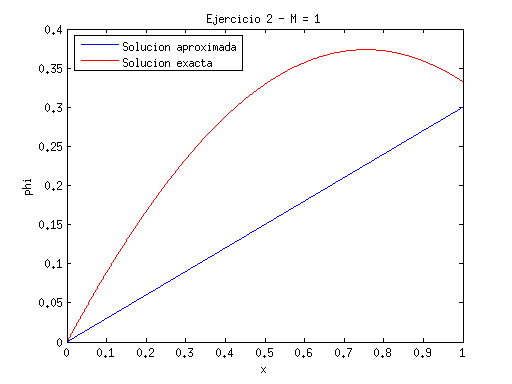
\includegraphics[width=\textwidth]{ej2_M_1.png}

        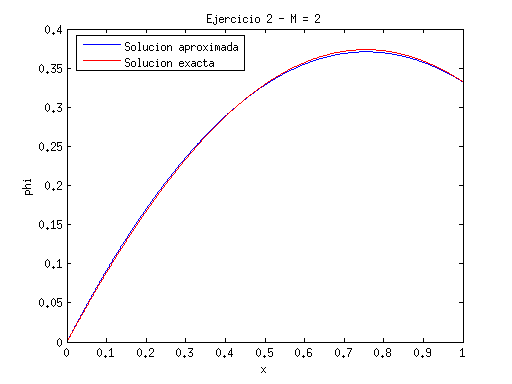
\includegraphics[width=\textwidth]{ej2_M_2.png}
    }
    \item{ % 3)
        La ecuación diferencial a resolver es

        \[ \frac{\partial^2 T}{\partial x^2} + \frac{\partial^2 T}{\partial y^2} = 0 \]

        con las condiciones de contorno

        \[ T(x, -1) = T(x, 1) = 1 - x^2 \]
        \[ T(-1, y) = T(1, y) = 1 - y^2 \]

        Aproximamos la solución con una función de la forma 
        $\hat{T} = \psi + \sum_{m=1}^M a_m N_m(x, y)$. Para satisfacer las condiciones 
        de contorno usamos

        \[ \psi = (1-x^2) + (1-y^2) \]

        y elegimos las funciones de forma de manera que se anulen en el contorno:

        \[ N_m = \sin\left(\frac{m \pi (x+1)}{2}\right) \sin\left(\frac{m \pi (y+1)}{2}\right) \]

        El residuo va a ser entonces

        \[ R_\Omega = \frac{\partial^2 \hat{T}}{\partial x^2} 
                      + \frac{\partial^2 \hat{T}}{\partial y^2} \]

        Usando Galerkin, la fórmula de residuos ponderados resultante es:

        \begin{eqnarray*}
        \intone\intone N_l \left[ \frac{\partial^2 \psi}{\partial x^2} 
        + \summ a_m \frac{\partial^2 N_m}{\partial x^2} 
        + \frac{\partial^2 \psi}{\partial y^2} 
        + \summ a_m \frac{\partial^2 N_m}{\partial y^2}\right] \dx\dy &=& 0 \\
        \summ a_m \left\{\intone\intone N_l \left[ \frac{\partial^2 N_m}{\partial x^2}
        + \frac{\partial^2 N_m}{\partial y^2}\right] \dx\dy  \right\}
        - 4 \intone\intone N_l \dx\dy &=& 0 \\
        \summ a_m \left\{\intone\intone N_l \left[ \frac{\partial^2 N_m}{\partial x^2}
        + \frac{\partial^2 N_m}{\partial y^2}\right] \dx\dy  \right\}
        &=& 4 \intone\intone N_l \dx\dy
        \end{eqnarray*}

        De donde se ve claramente que:

        \[ K_{lm} = \intone\intone N_l \left[ \frac{\partial^2 N_m}{\partial x^2}
        + \frac{\partial^2 N_m}{\partial y^2}\right] \dx\dy \]
        \[ f_l = 4 \intone\intone N_l \dx\dy \]

        Usando dos de las funciones de forma antes mencionadas se obtiene el siguiente
        resultado: 

        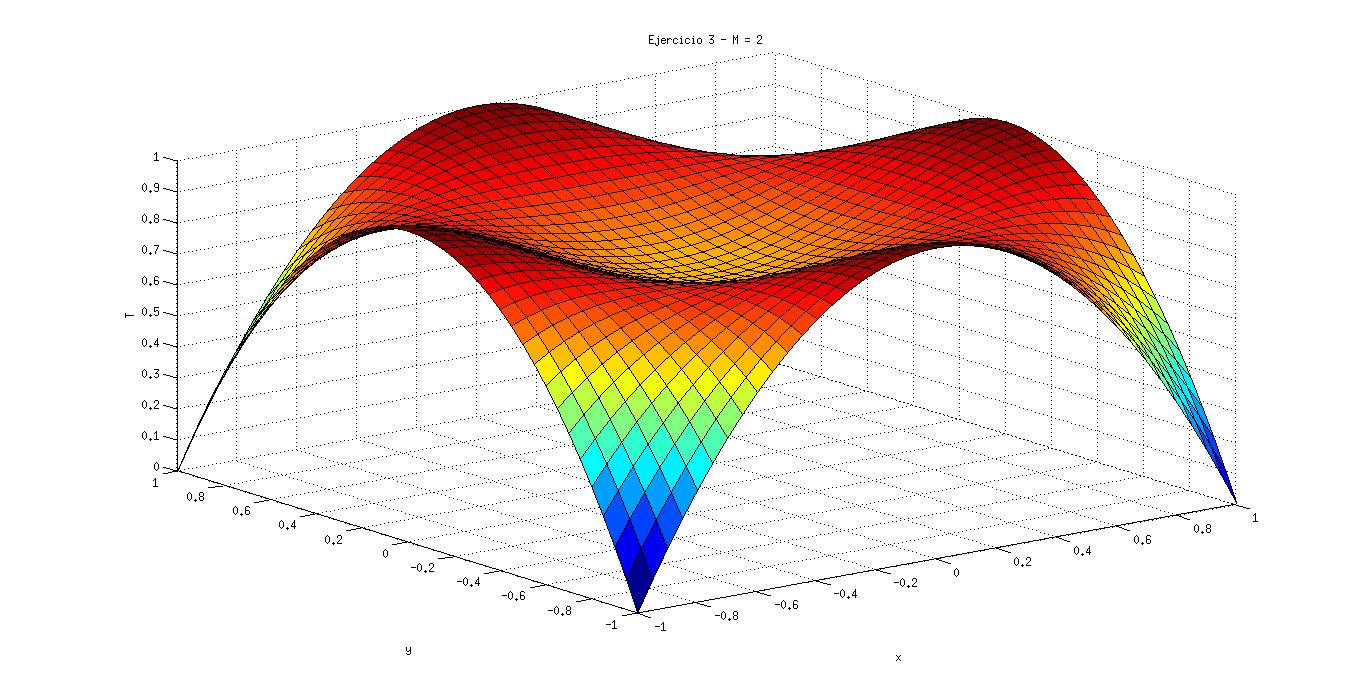
\includegraphics[width=\textwidth]{ej3.png}
    }
    \item{ % 4)
        El problema está dado por la ecuación de equilibrio

        \[ \partialx{\sigma_x} + \partialy{\tau_{xy}} - b_x = 0 \]

        Hay condiciones de borde Dirichlet (en los bordes superior e inferior) y Neumann (en los
        bordes izquierdo y derecho). Las Dirichlet son simplemente

        \[ \boldsymbol{u} = \boldsymbol{0} \qquad \mbox{en $y = \pm 1$} \]

        O sea, las aristas en $y = \pm 1$ están fijas. Las condiciones Neumann son

        \[ \sigma_x n_x + \tau_{xy} n_y - \bar{t}_x = 0 \]

        donde $\bar{t}_x = \frac{E (1-y^2)}{1 + \nu}$

        En este caso la solución que se busca (los desplazamientos) tiene dos componentes. Se aproxima de la forma
        
        \[ \boldsymbol{\psi} \approx \boldsymbol{\hat{\psi}} = \left[ \begin{array}{c} \hat{u} \\ \hat{v} \end{array} \right] \]

        donde

        \[ \hat{u} = \psi_1 + \summ a_m N_m \]
        \[ \hat{v} = \psi_2 + \summ a_m N_m \]

        Por comodidad, trabajamos sólo con el componente $u$. Además, como las funciones de 
        peso para $u$ y para $v$ pueden ser distintas, hay un grupo de funciones $w_{l,1}$ y 
        otro $w_{l, 2}$, además de los equivalentes usados en el contorno, pero se usará
        $w_l$ en su lugar.

        Las condiciones Dirichlet se satisfacen simplemente haciendo $\psi_1 = \psi_2 = 0$. Las
        condiciones Neumann se incluyen en el residuo. El método toma la forma

        \[ 
            \int_\Omega \left( \partialx{\hatsigmax} + \partialx{\hattauxy} - b_x \right) W_l \domega 
            +
            \int_\Gamma \left( \hatsigmax n_x + \hattauxy n_y - \bar{t}_x \right) \bar{W_l} \dgamma = 0
        \]

        Como las tensiones involucran una derivada de primer orden de los desplazamientos (a través
        de las deformaciones), nuestra ecuación involucra derivadas de segundo orden de la incógnita.
        Para evitar esto, debilitamos aplicando la ley de Green y obtenemos

        \begin{eqnarray*}
            &-&\int_\Omega \left[ 
            \hatsigmax \partialx{W_l} + \hattauxy \partialy{W_l} - W_l b_x
            \right] \domega + \\
            &+&
            \int_{\Gamma_u + \Gamma_t} \left[ 
            \hatsigmax n_x + \hattauxy n_y
            \right] W_l \dgamma
            +
            \int_{\Gamma_t} \left[ 
            \hatsigmax n_x + \hattauxy n_y - \bar{t}_x
            \right] \bar{W_l} \dgamma
            = 0
        \end{eqnarray*}

        Donde $\Gamma_t$ es la frontera con condiciones Neumann y $\Gamma_u$ es la frontera con
        condiciones Dirichlet. Haciendo $\bar{W}_l = - W_l$ y garantizando que $W_l$ se anule
        en $\Gamma_u$ la ecuación se reduce a

        \[
            -\int_\Omega \left[ 
            \hatsigmax \partialx{W_l} + \hattauxy{W_l} - W_l b_x
            \right] \domega
            +
            \int_{\Gamma_t} \bar{t}_x W_l \dgamma = 0
        \]

        Para $v$ se obtiene una expresión similar (donde $W_l$ en este contexto quiere decir
        $W_{l,2}$)

        \[
            -\int_\Omega \left[ 
            \hattauxy{W_l} + \hatsigmay \partialy{W_l} - W_l b_y
            \right] \domega
            +
            \int_{\Gamma_t} \bar{t}_y W_l \dgamma = 0
        \]

        Ambos resultados pueden combinarse en uno solo en forma matricial:

        \[
            \int_\Omega 
            \left(\boldsymbol{\mathcal{L}} \boldsymbol{W_l}\right)^T
            \boldsymbol{D} \boldsymbol{\mathcal{L}} \boldsymbol{\hat{\phi}} \domega
            +
            \int_{\Gamma_t} \boldsymbol{W_l} \boldsymbol{t} \dgamma = \boldsymbol{0}
        \]

        Donde

        \[ \boldsymbol{\mathcal{L}} = 
           \left[ \begin{array}{cc} 
               \partialx{} & 0 \\ 
               0 & \partialy{} \\
               \partialy{} & \partialx{}
            \end{array} \right] \]

        \[ \boldsymbol{W_l} = 
           \left[ \begin{array}{cc} 
               W_{l,1} & 0 \\ 
               0 & W_{l,2}
            \end{array} \right] \]

        \[ \boldsymbol{D} = 
           \frac{E}{1-\nu^2}
           \left[ \begin{array}{ccc} 
               1 & \nu & 0 \\ 
               \nu & 1 & 0 \\ 
               0 & 0 & \frac{1-\nu}{2}
            \end{array} \right] \]

        Donde $\boldsymbol{\hat{\phi}} = \boldsymbol{\psi} + \summ a_m \boldsymbol{N_m}$.
        Si desarrollamos este término y agrupamos, obtenemos las componentes del
        SEAL resultante:

        \[ K_{lm} = \int_\Omega 
            \left(\boldsymbol{\mathcal{L}} \boldsymbol{W_l}\right)^T
            \boldsymbol{D} \boldsymbol{\mathcal{L}} \boldsymbol{N_m} \domega\]

        \[ f_l = \int_\Omega \boldsymbol{W_l} \boldsymbol{b} \domega + 
            \int_{\Gamma_t} \boldsymbol{W_l} \boldsymbol{t} \dgamma -
            \int_\Omega 
            \left(\boldsymbol{\mathcal{L}} \boldsymbol{W_l}\right)^T
            \boldsymbol{D} \boldsymbol{\mathcal{L}} \boldsymbol{\psi} \domega\]


    }
\end{enumerate}
\end{document}
